\documentclass{beamer}
\usepackage{luatexja}
\usepackage[mark=o]{dynkin-diagrams}
\usetheme[block=fill]{metropolis}
\usecolortheme{seahorse}
\theoremstyle{definition}
\newtheorem{proposition}{Proposition}

\title{Onsager代数の話}
\subtitle{Generalized Onsager algebras}
\author{宇佐見 公輔}
\date{2019年8月3日}
\begin{document}

\begin{frame}
    \titlepage{}
\end{frame}

\begin{frame}
    \frametitle{Onsager algebra とは}

    \begin{itemize}
        \item \(\mathbb{C}\) 上の無限次元リー代数
        \item 1944年、L. Onsager が2次元 Ising model を解くため導入
        \item 1980〜90年代ごろに研究が進み、注目されはじめる
        \item Ising model 以外の各種の数理物理のモデルへの応用も
    \end{itemize}
\end{frame}

\begin{frame}
    \frametitle{2次元 Ising model}

    \begin{columns}[c]
        \begin{column}{0.7\linewidth}
            \begin{itemize}
                \item \(m \times n\) の格子模型
                \item 各点で \(\pm 1\) の値(スピン)を持つ
                \item 温度が下がると隣接点が同じスピンに揃いたがる(そのようにハミルトニアンを定義する)
                \item 1944年に Onsager algebra で解かれた(その後もう少し分かりやすい手法で解かれた)
                \item なお、3次元以上では解法は見つかっていない
            \end{itemize}
        \end{column}
        \begin{column}{0.3\linewidth}
            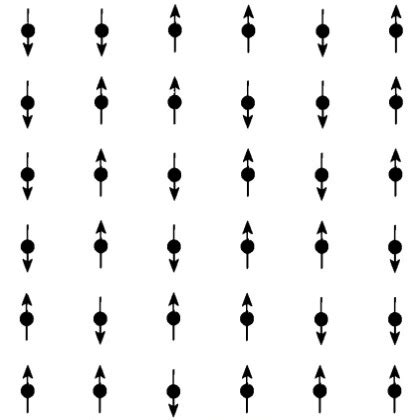
\includegraphics[width=\linewidth]{images/ising.jpeg}
        \end{column}
    \end{columns}
\end{frame}

\begin{frame}
    \frametitle{Onsager algebra の研究}

    \begin{itemize}
        \item 1980〜90年代ごろ、同型な対応がいくつか見つかる
        \item 特に、アフィンリー代数との関連が見つかる
        \item そこから、q-Onsager algebra や、Onsager algebra の一般化が研究される
        \item 今回は Onsager algebra の一般化について触れる
    \end{itemize}
\end{frame}

\begin{frame}
    \frametitle{Onsager algebra の定義}

    \begin{definition}[Onsager algebra]
        \( \{A_m, G_m\} \) (\( m \in \mathbb{Z} \)) を基底として持ち、
        ブラケット積を以下で定義したリー代数を Onsager algebra という。
        \begin{align*}
            [A_m, A_n] & = 4G_{m-n}            \\
            [G_m, A_n] & = 2A_{m+n} - 2A_{m-n} \\
            [G_m, G_n] & = 0
        \end{align*}
    \end{definition}
\end{frame}

\begin{frame}
    \frametitle{Dolan-Grady 関係式}

    \begin{proposition}[Dolan-Grady 関係式]
        Onsager algebra は、生成元 \(A_0, A_1\) と
        以下の関係式で生成されるリー代数と同型である。
        \begin{align*}
            [A_0, [A_0, [A_0, A_1]]] & = 16[A_0, A_1] \\
            [A_1, [A_1, [A_1, A_0]]] & = 16[A_1, A_0] \\
        \end{align*}
    \end{proposition}

    こちらを Onsager algebra の定義としても差し支えない。
\end{frame}

\begin{frame}
    \frametitle{loop algebra の involution}

    loop algebra \(\mathbb{C}[t,t^{-1}] \otimes \mathfrak{sl}(2,\mathbb{C})\) を考える。
    ここで \(\mathbb{C}[t,t^{-1}]\) は変数 \(t\) のローラン多項式である。

    \begin{definition}[loop algebra の involution]
        \(\mathfrak{sl}(2,\mathbb{C})\) の involution \(\omega \) を以下で定義する。
        \begin{align*}
            e & \mapsto f  \\
            f & \mapsto e  \\
            h & \mapsto -h
        \end{align*}
        \(\mathbb{C}[t,t^{-1}] \otimes \mathfrak{sl}(2,\mathbb{C})\) 上の
        involution \(\omega \) を以下で定義する。
        \[
            p(t) \otimes x \mapsto p(t^{-1}) \otimes \omega(x)
        \]
    \end{definition}
\end{frame}

\begin{frame}
    \frametitle{loop algebra の fixed point subalgebra}

    \begin{proposition}[loop algebra の fixed point subalgebra]
        \(\mathbb{C}[t,t^{-1}] \otimes \mathfrak{sl}(2,\mathbb{C})\) の部分リー代数
        \[
            \{ x \in \mathbb{C}[t,t^{-1}] \otimes \mathfrak{sl}(2,\mathbb{C}) \mid \omega(x) = x \}
        \]
        (\(\omega \) による fixed point subalgebra)は Onsager algebra と同型である。
        また、以下の \( \{A_m, G_m\} \) (\( m \in \mathbb{Z} \)) がその基底である。
        \begin{align*}
            A_m & = 2t^m e + 2t^{-m} f \\
            G_m & = (t^m - t^{-m}) h
        \end{align*}
    \end{proposition}

    Onsager algebra は \(A_1^{(1)}\) 型のアフィンリー代数
    (= loop algebra \(\mathbb{C}[t,t^{-1}] \otimes \mathfrak{sl}(2,\mathbb{C})\) の中心拡大)
    の部分リー代数ともいえる。
\end{frame}

\begin{frame}
    \frametitle{Onsager algebra の拡張の発想}

    \begin{itemize}
        \item Onsager algebra は \(A_1^{(1)}\) 型のアフィンリー代数の部分リー代数であることがわかった
        \item では、\(A_1^{(1)}\) 型以外のアフィンリー代数を考えれば、
              Onsager algebra の拡張を考えられるのではないか?
    \end{itemize}
\end{frame}


\begin{frame}
    \frametitle{\(A_n^{(1)}\) への拡張}

    Uglov と Ivanov による A 型への拡張(1996)

    \begin{definition}[A 型 Onsager algebra]
        生成元 \(e_0, \dots, e_n\) と以下の関係式で生成されるリー代数を \(A_n^{(1)}\) 型 Onsager algebra と呼ぶ。
        \begin{align*}
            [e_i, [e_i, e_j]] & = e_j & \quad & \text{Dynkin 図形上で頂点が隣のとき} \\
            [e_i, [e_i, e_j]] & = 0   & \quad & \text{otherwise}
        \end{align*}

        上記の Dynkin 図形は \(A_n^{(1)}\) 型のもの。

        \scalebox{2}{
            \dynkin[extended]{A}{}
        }
    \end{definition}
\end{frame}

\begin{frame}
    \frametitle{関係式の意味}

    A 型 Onsager algebra の関係式
    \[
        [e_i, [e_i, e_j]] = e_j
    \]
    は、A 型有限次元単純リー代数の Serre 関係式
    \[
        [e_i, [e_i, e_j]] = 0
    \]
    の類似と考えられる。

    また、Onsager algebra の Dolan-Grady 関係式
    \[
        [A_i, [A_i, [A_i, A_j]]] = 16[A_i, A_j]
    \]
    の類似と考えられる。
\end{frame}

\begin{frame}
    \frametitle{loop algebra の fixed point subalgebra}

    \begin{proposition}[loop algebra の fixed point subalgebra]
        \(\mathbb{C}[t,t^{-1}] \otimes \mathfrak{sl}(n,\mathbb{C})\) の
        involution \(\omega \) を以下で定義する。
        \begin{align*}
            t^m E_{ij} & \mapsto {(-1)}^{i+j+1+mn} t^{-m} E_{ji} \\
            t^m H_i    & \mapsto {(-1)}^{1+mn} t^{-m} H_i
        \end{align*}

        \(\mathbb{C}[t,t^{-1}] \otimes \mathfrak{sl}(n+1,\mathbb{C})\) の
        fixed point subalgebra は \(A_n^{(1)}\) 型 Onsager algebra と同型である。
    \end{proposition}

    \(A_n^{(1)}\) 型 Onsager algebra は \(A_n^{(1)}\) 型のアフィンリー代数の部分リー代数ともいえる。
\end{frame}

\begin{frame}
    \frametitle{\(D_n^{(1)}\) への拡張}

    Date と Usami による D 型への拡張(2004)

    \begin{definition}[D 型 Onsager algebra]
        生成元 \(e_0, \dots, e_n\) と以下の関係式で生成されるリー代数を \(D_n^{(1)}\) 型 Onsager algebra と呼ぶ。
        \begin{align*}
            [e_i, [e_i, e_j]] & = e_j & \quad & \text{Dynkin 図形上で頂点が隣のとき} \\
            [e_i, [e_i, e_j]] & = 0   & \quad & \text{otherwise}
        \end{align*}

        上記の Dynkin 図形は \(D_n^{(1)}\) 型のもの。

        \scalebox{2}{
            \dynkin[extended]{D}{}
        }
    \end{definition}
\end{frame}

\begin{frame}
    \frametitle{loop algebra の fixed point subalgebra}

    \begin{proposition}[loop algebra の fixed point subalgebra]
        \(\mathbb{C}[t,t^{-1}] \otimes \mathfrak{o}(2n,\mathbb{C})\) の
        involution \(\omega \) を以下で定義する。
        \[
            t^m G_{ij} \mapsto {(-1)}^{\alpha(i,j)} t^{-m} G_{ji}
        \]
        (\(G_{ij} := E_{ij} - E_{2n+1-j,2n+1-i}\)、\(\alpha(i,j) := i+j \text{または} i+j+1\))

        \(\mathbb{C}[t,t^{-1}] \otimes \mathfrak{o}(2n,\mathbb{C})\) の
        fixed point subalgebra は \(D_n^{(1)}\) 型 Onsager algebra と同型である。
    \end{proposition}

    \(D_n^{(1)}\) 型 Onsager algebra は \(D_n^{(1)}\) 型のアフィンリー代数の部分リー代数ともいえる。
\end{frame}

\begin{frame}
    \frametitle{Generalized Onsager algebra}

    Stokman による一般の Kac-Moody algebra への拡張(2019)

    \begin{definition}[Generalized Onsager algebra]
        \(A = (a_{ij})\) を対称化可能な generalized Cartan matrix とする。
        生成元 \(e_1, \dots, e_n\) と以下の関係式で生成されるリー代数を Generalized Onsager algebra と呼ぶ。
        \[
            \sum_{s=0}^{1-a_{ij}} c_s^{ij}[1-a_{ij}] {(\mathrm{ad} e_i)}^s e_j = 0
        \]
    \end{definition}

    \begin{itemize}
        \item Cartax matrix が \(A_1^{(1)}\) 型の場合は Dolan-Grady 関係式
        \item \(A_n^{(1)}\) 型の場合は Uglov と Ivanov の定義
        \item \(D_n^{(1)}\) 型の場合は Date と Usami の定義
    \end{itemize}
    に、それぞれ一致する。
\end{frame}

\begin{frame}
    \frametitle{まとめ}

    \begin{itemize}
        \item 以前やっていたことが一般化された論文が出ていて驚いた、
        \item しかもその論文の中に自分の名前が出てきてさらに驚いた、
    \end{itemize}
    というお話でした。

    参考文献:
    \begin{itemize}
        \item Generalized Onsager algebras, Jasper V. Stokman, preprint, 2019
    \end{itemize}
\end{frame}

\end{document}
